\documentclass[11pt]{article}
\usepackage{latexsym}
\usepackage{amsmath}
\usepackage{amssymb}
\usepackage{amsthm}
\usepackage{epsfig}
\usepackage[tight]{subfigure}
\usepackage{subcaption}
\usepackage{amsmath}

\DeclareMathOperator*{\minimize}{min}
\DeclareMathOperator*{\maximize}{max}
\DeclareMathOperator*{\argmax}{arg\,max}
\DeclareMathOperator*{\argmin}{arg\,min}
\usepackage{algorithm}
 %on linux you may need to run sudo apt-get install texlive-full to install algorithm.sys
\usepackage{algorithmic}

\usepackage{verbatim}

\newcommand{\handout}[5]{
  \noindent
  \begin{center}
  \framebox{
    \vbox{
      \hbox to 5.78in { {#1} \hfill #2 }
      \vspace{4mm}
      \hbox to 5.78in { {\Large \hfill #5  \hfill} }
      \vspace{2mm}
      \hbox to 5.78in { {\em #3 \hfill #4} }
    }
  }
  \end{center}
  \vspace*{4mm}
}

\newcommand{\lecture}[5]{\handout{#1}{#2}{#3}{#4}{#5}}
\newcommand{\collision}[0]{\mathrm{collision}}
\newcommand{\nocollision}[0]{\overline{\collision}}

\newcommand*{\QED}{\hfill\ensuremath{\square}}

\newtheorem{theorem}{Theorem}
\newtheorem{corollary}[theorem]{Corollary}
\newtheorem{lemma}[theorem]{Lemma}
\newtheorem{observation}[theorem]{Observation}
\newtheorem{proposition}[theorem]{Proposition}
\newtheorem{definition}[theorem]{Definition}
\newtheorem{claim}[theorem]{Claim}
\newtheorem{fact}[theorem]{Fact}
\newtheorem{assumption}[theorem]{Assumption}
\newtheorem{note}[theorem]{Note}


\newcommand{\norm}[1]{\left\lVert#1\right\rVert}
\usepackage{bbm}


% 1-inch margins, from fullpage.sty by H.Partl, Version 2, Dec. 15, 1988.
\topmargin 0pt
\advance \topmargin by -\headheight
\advance \topmargin by -\headsep
\textheight 8.9in
\oddsidemargin 0pt
\evensidemargin \oddsidemargin
\marginparwidth 0.5in
\textwidth 6.5in

\parindent 0in
\parskip 1.5ex
%\renewcommand{\baselinestretch}{1.25}

\begin{document}

\lecture{Statistical Techniques in Robotics (16-831, S20)}{Lecture \#10
  (Monday, March 08)}{Lecturer: Kris Kitani}{Scribes: Paritosh Mittal, Tanay Sharma}{ Hard-SVM, Soft-SVM, OSGD }

\section{Review}
Last lecture introduced the concept of Gradient Descent and Stochastic Gradient Descent. It further explained how Online Gradient Descent is a special case of Online Mirror Descent (OMD). In this section, we will review these topics and develop tools that can be used to solve optimization problem for Max Margin Classifier (SVM). We will cover the (1) definition of convex functions, (2) Gradient Descent and (3) its links with OMD.
\subsection{Convex Functions}
A function $f : S \to \mathbb{R}$ is convex if for all $\mathbf{w,v} \in S$
\[ 
f(\alpha\mathbf{w} + (1-\alpha)\mathbf{v}) \leq \alpha f(\mathbf{w}) + (1-\alpha)f(\mathbf{v})
\]
\[
\text{for all }\alpha \in [0,1]
\]
Key properties of a convex smooth bounded function include (1) we can find the global minimum and (2) we can find it fast(er). We can formulate a convex optimization problem with a convex function and a convex solution space. However, the convex function needs to be convex-Lipschitz-bounded or convex-smooth-bounded.

\subsection{Gradient Descent}
Gradient Descent is an approach for minimizing differentiable (or non-differentiable in case of sub gradient descent) convex functions with regularization as added constraint. \begin{figure}[!b]
    \centering
    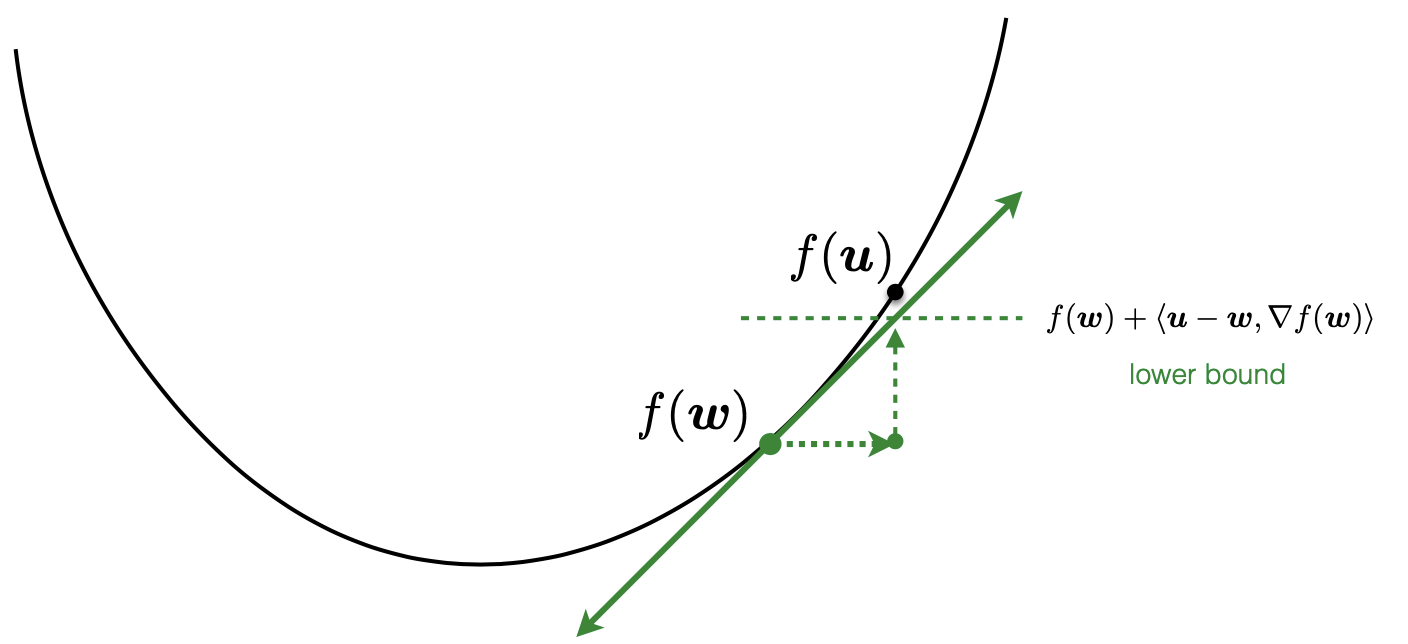
\includegraphics[width=0.5\linewidth]{images/GD_Taylor_Approx.png}
    \caption{Taylor Series approximation of $f(\mathbf{u})$}
    \label{fig:1}
\end{figure}
Consider a convex function $f$ in figure \ref{fig:1}, wherein we use Taylor series approximation of $1^{st}$ order, to lower bound $f(\mathbf{u})$
\[
f(\mathbf{u}) \geq f(\mathbf{w}) + \langle\mathbf{u}-\mathbf{w},\nabla f(\mathbf{w})\rangle
\]
If we directly select $\mathbf{u}$ that minimize $f$ using only the previous inequality then we get solution at negative infinity. To avoid this we introduce a regularization term that constraints $\mathbf{w}$ to be close to $\mathbf{u}$. The final objective function for gradient descent hence looks like:
\begin{equation}
    \label{eq:1}
    \mathbf{w}^{(t+1)} = \argmin_{\mathbf{w}} \frac{1}{2} ||\mathbf{w} - \mathbf{w}^{(t)}||^2 + \eta (f(\mathbf{w}^{(t)}) + \langle\mathbf{w}-\mathbf{w}^{(t)},\nabla f(\mathbf{w}^{(t)})\rangle
\end{equation}
where $\eta$ is a Lagrangian multiplier. Here we use gradient descent to solve the objective function in equation \ref{eq:1}. If we observe closely then equation \ref{eq:1} is of the form of quadratic regularization + linear loss function. We know from past lectures that OMD solve objective functions with linear loss with quadratic regularization.
\subsection{Online Gradient Descent(OGD): Special case of OMD}
OMD is often used to solve optimization problems that contain a linear loss function $f(\mathbf{w})$ and a quadratic regularization $\psi(\mathbf{w})$. In case of OGD, we can write them as:
\[ \psi(\mathbf{w}) = \frac{1}{2\eta} ||\mathbf{w}||_2^2 \text{  and  } f(\mathbf{w}) = \langle \mathbf{w},\pmb{\theta} \rangle
\]
Where $\pmb{\theta}$ is the parameter for dual space. We can see that $f(\mathbf{w})$ is linear and $\psi(\mathbf{w})$ is quadratic for OGD. Further when we solve for optimal parameter to minimize the convex function, we notice
\[
w_n = \eta \theta
\]
Hence the mirror function for OGD is $g(\pmb{\theta}) = \eta \pmb{\theta}$. Therefore OGD is OMD with a linear loss $\&$ quadratic regularization (or quadratic loss with linear constraints). We will soon notice that optimization problem for max-margin classifier (SVM) is of similar form and hence OGD can be used to solve it.
\section{Summary}
\subsection{Hyperplanes}
A hyperplane of an n-dimensional vector space is geometrically defined as a subspace of dimension n-1 \cite{Hyperplane_def}. In simple terms, a hyperplane of 2D vector space is a line and that of a 3D vector space is a 2D plane. Mathematically, hyperplane is defined as 
\[
\mathbf{w} \cdot \mathbf{x} + b = 0 \text{    where } \mathbf{w} \in \mathcal{R}^n \text{ for n dimensional space}
\]
Key observations for hyperplane include
\begin{itemize}
    \item \textbf{We can choose any normalization of w}: Equality in hyperplanes are to scale, i.e. if we multiply an equation of hyperplane with non-zero factor $\lambda$ then we get the same hyperplane
    \[w_1 x_1 + w_2x_2 +b = 0 \text{  and  } \lambda(w_1 x_1 + w_2x_2 + b) = 0 \text{ correspond to same hyperplanes}\]
    \item \textbf{Distance of hyperplane from origin}: The perpendicular distance of a hyperplane $\mathbf{w \cdot x} + b = 0$ from the origin of n-dimensional vector space is $b/||\mathbf{w}||$
    \[
    \text{if we scale:  } \mathbf{w \cdot x} + b = 0 \text{ with } \frac{1}{||\mathbf{w}||} 
    \]
    \[
    \text{transformed to normal form:  } x \cos \theta + y \sin \theta = \rho
    \]
    \[
    \text{we get distance from origin:   } \rho = \frac{b}{||\mathbf{w}||}
    \]
    \item \textbf{Distance between parallel hyperplanes}: Consider two parallel hyperplanes defined by (a) $\mathbf{w \cdot x} + b = 1$ and (b) $\mathbf{w \cdot x} + b = -1$
    \begin{equation*}
        \begin{split}
            \text{  distance of hyperplane (a) from origin:  }& \frac{b-1}{||\mathbf{w}||}\\
            \text{  distance of hyperplane (b) from origin:   }& \frac{b+1}{||\mathbf{w}||}\\
            \text{perpendicular distance between these hyperplanes:}& \frac{2}{||\mathbf{w}||}
        \end{split}
    \end{equation*}
\end{itemize}
Note that because we can choose any normalization of $\mathbf{w}$ for the hyperplanes, we can always write the distance between two parallel hyperplanes as $2/||\mathbf{w}||$. This is hence used as convention (fig. \ref{fig:2}).
\begin{figure}[!t]
    \centering
    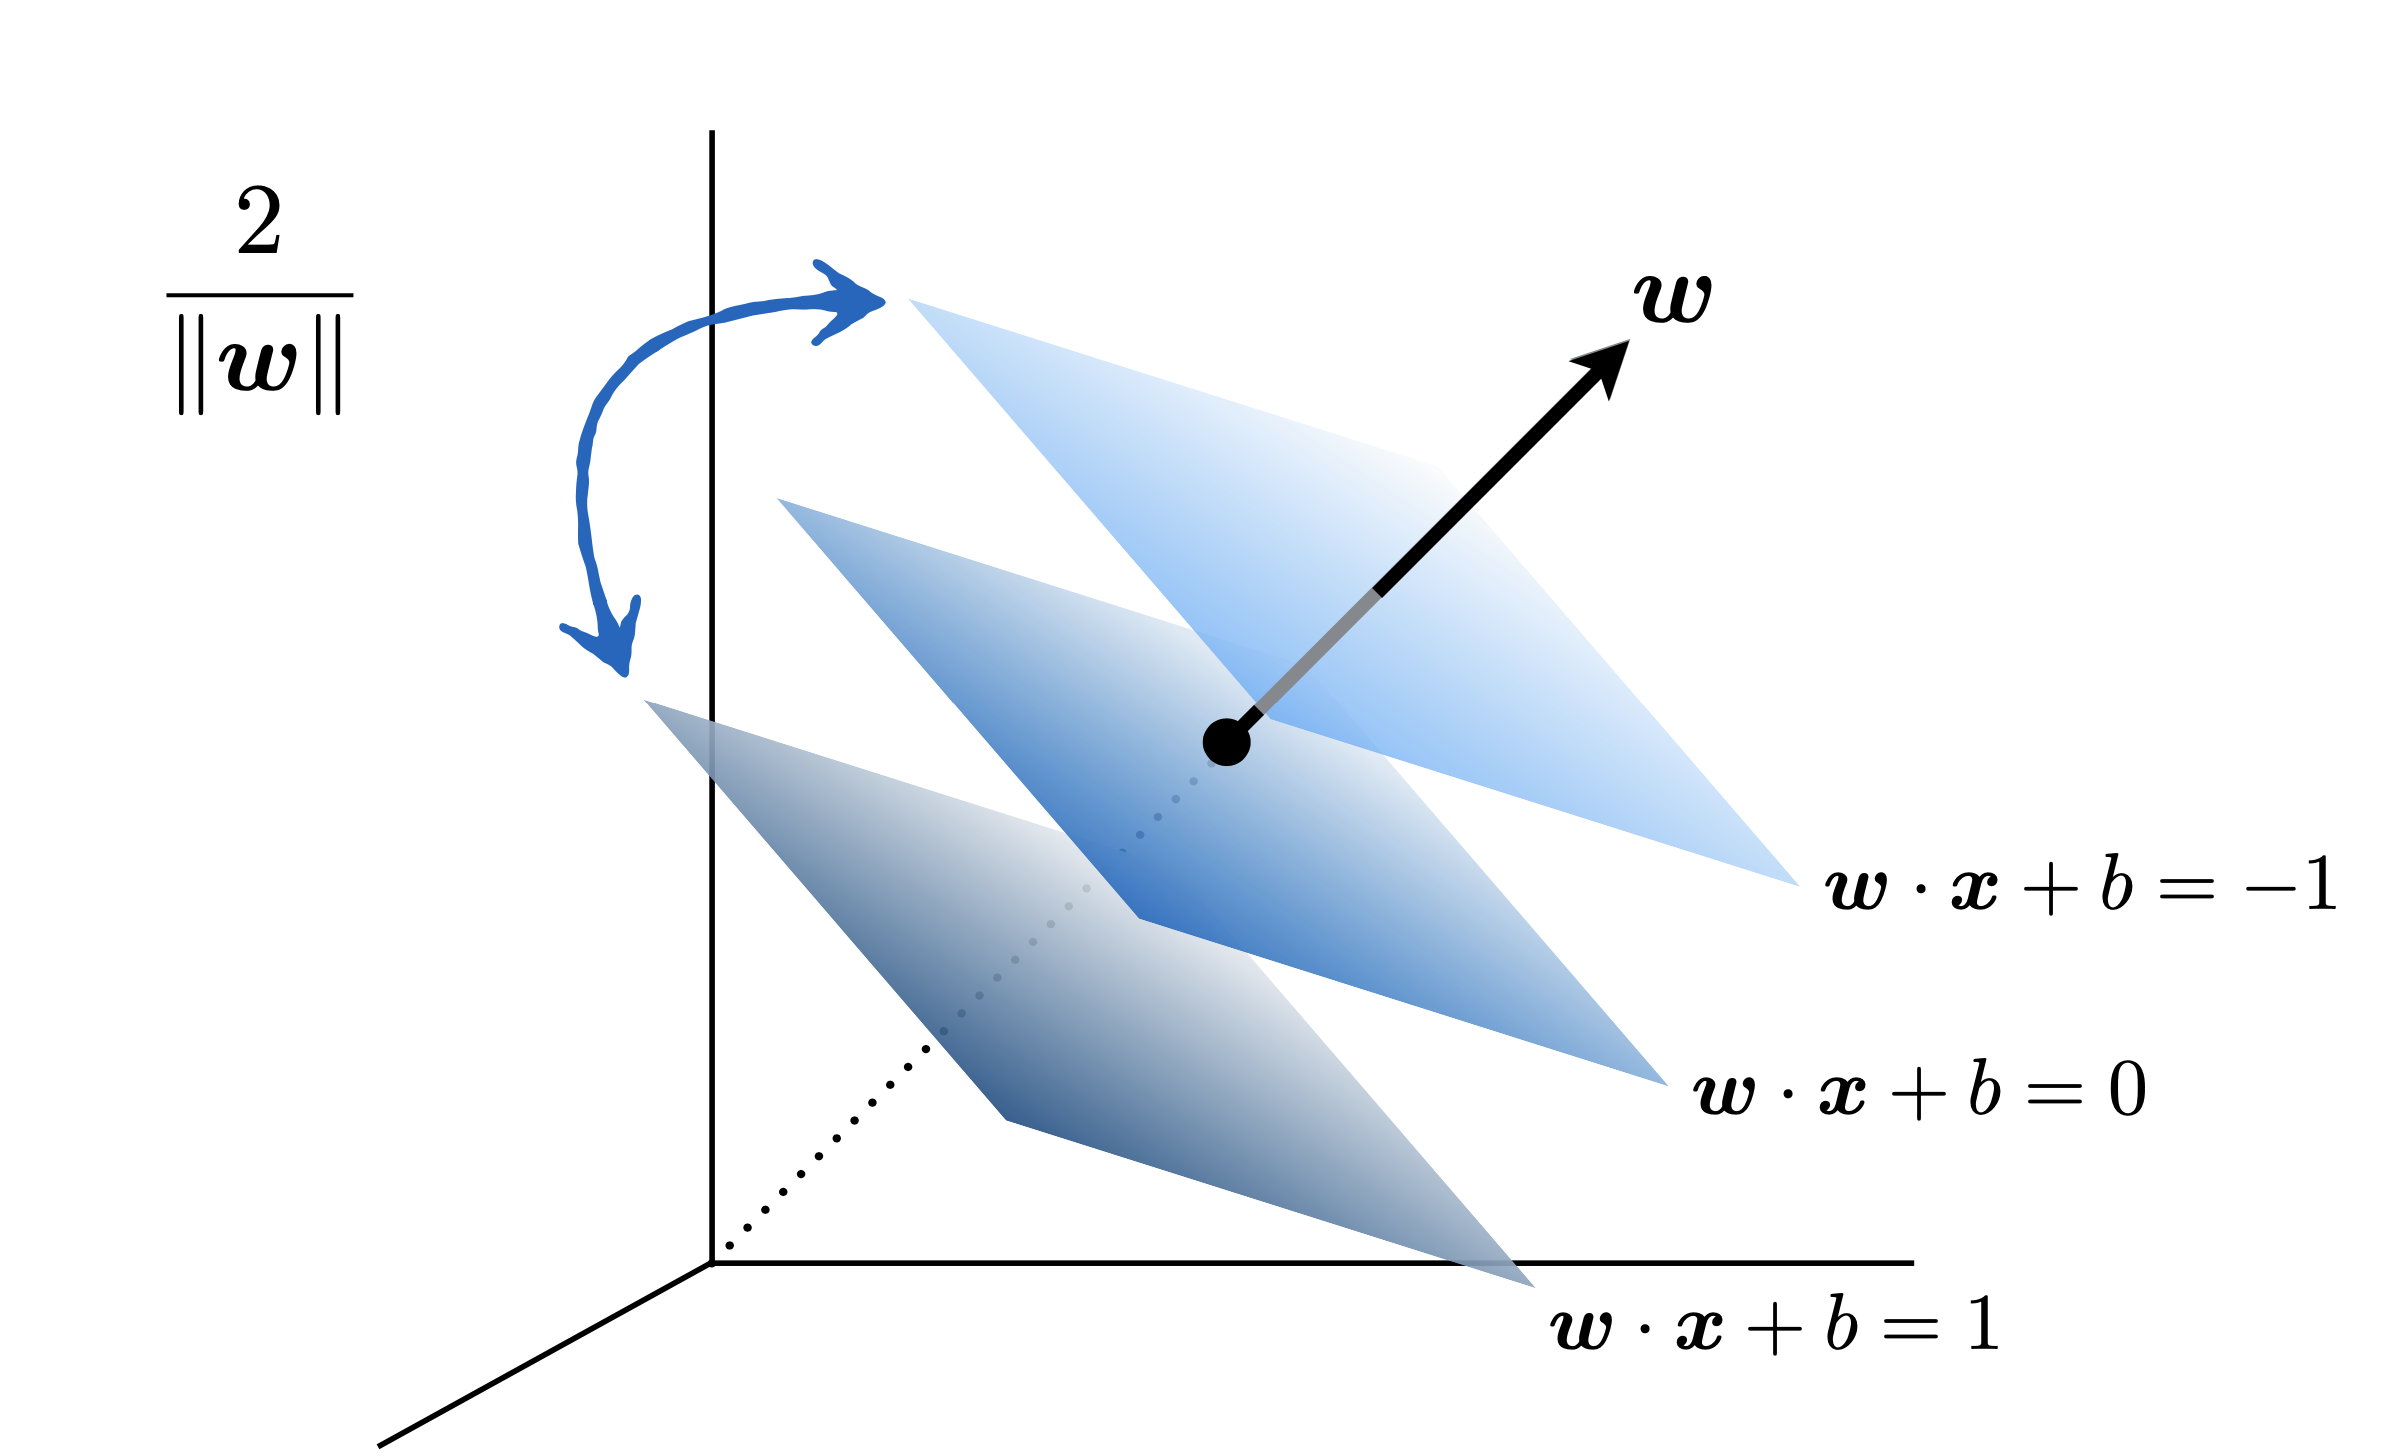
\includegraphics[width=0.5\linewidth]{images/Distance_between_hyperplanes.png}
    \caption{Distance between parallel hyperplanes}
    \label{fig:2}
\end{figure}
\subsection{Support Vector Machine (Max Margin Classifier)}
Consider a case of binary linearly separable data ($\mathcal{D}$), the task at hand is to learn a linear decision boundary that perfectly classifies this data. We know from our knowledge of Perceptron, that there are infinite such hyperplanes possible for linearly separable data. However, Max Margin Classifier learns a decision boundary (surface) with maximum margin ($\gamma$).
\definition{\textbf{Margin}($\gamma$) of a set of points in $\mathcal{D}$ is defined as the distance from the decision surface to the closest point in $\mathcal{D}$.}\\
\normalfont
Refer to figure \ref{fig:3} for better visualization. Without loss of generality, let $\mathbf{w \cdot x} + b = 0$ be the equation for max-margin classifier such that parallel hyperplanes $\mathbf{w \cdot x} + b = 1 \text{ and } \mathbf{w \cdot x} + b = -1$ pass through the nearest data points to classifier hyperplane. The distance between these planes correspond to the margin of the classifier. Hence we know that margin for linearly separable data with decision boundary $\mathbf{w \cdot x} + b = 0$ is 
\[
\frac{2}{||\mathbf{w}||}
\]
Hence the objective of the max-margin classifier is 
\begin{equation*}
    \begin{split}
        \maximize_{\mathbf{w}}& \frac{2}{||\mathbf{w}||} \:\: \text{   subject to}\\
        \mathbf{w \cdot x} +& b
        \begin{cases}
            \geq +1 &\text{ if } y_i = +1\\
            \leq -1 &\text{ if } y_i = -1
        \end{cases}
        \text{ for  } x_i \in \mathcal{D}
    \end{split}
\end{equation*}
Equivalently, we can simplify the problem as 
\begin{equation*}
    \begin{split}
        \minimize_{\mathbf{w}}& ||\mathbf{w}||^2\\
        \text{ subject to } y_i(\mathbf{w \cdot x_i + b}& \geq 1) \text{ for } i = 1,\cdots, N 
    \end{split}
\end{equation*}
We identify $\minimize_{\mathbf{w}} ||\mathbf{w}||^2$ as the objective function and $y_i(\mathbf{w \cdot x_i + b})& \geq 1$ as the ``Hard" constraints. There exists a unique solution for this problem and we can use tools of convex quadratic programming (QP) problem to solve it. \\
We make a major assumption here that data ($\mathcal{D}$) is linearly separable, this is generally not the case for most real life scenarios. To counter this problem there is a popular variant of SVMs termed as ``Soft" SVMs which allow for some `slack'.
\begin{figure}[!t]
    \centering
    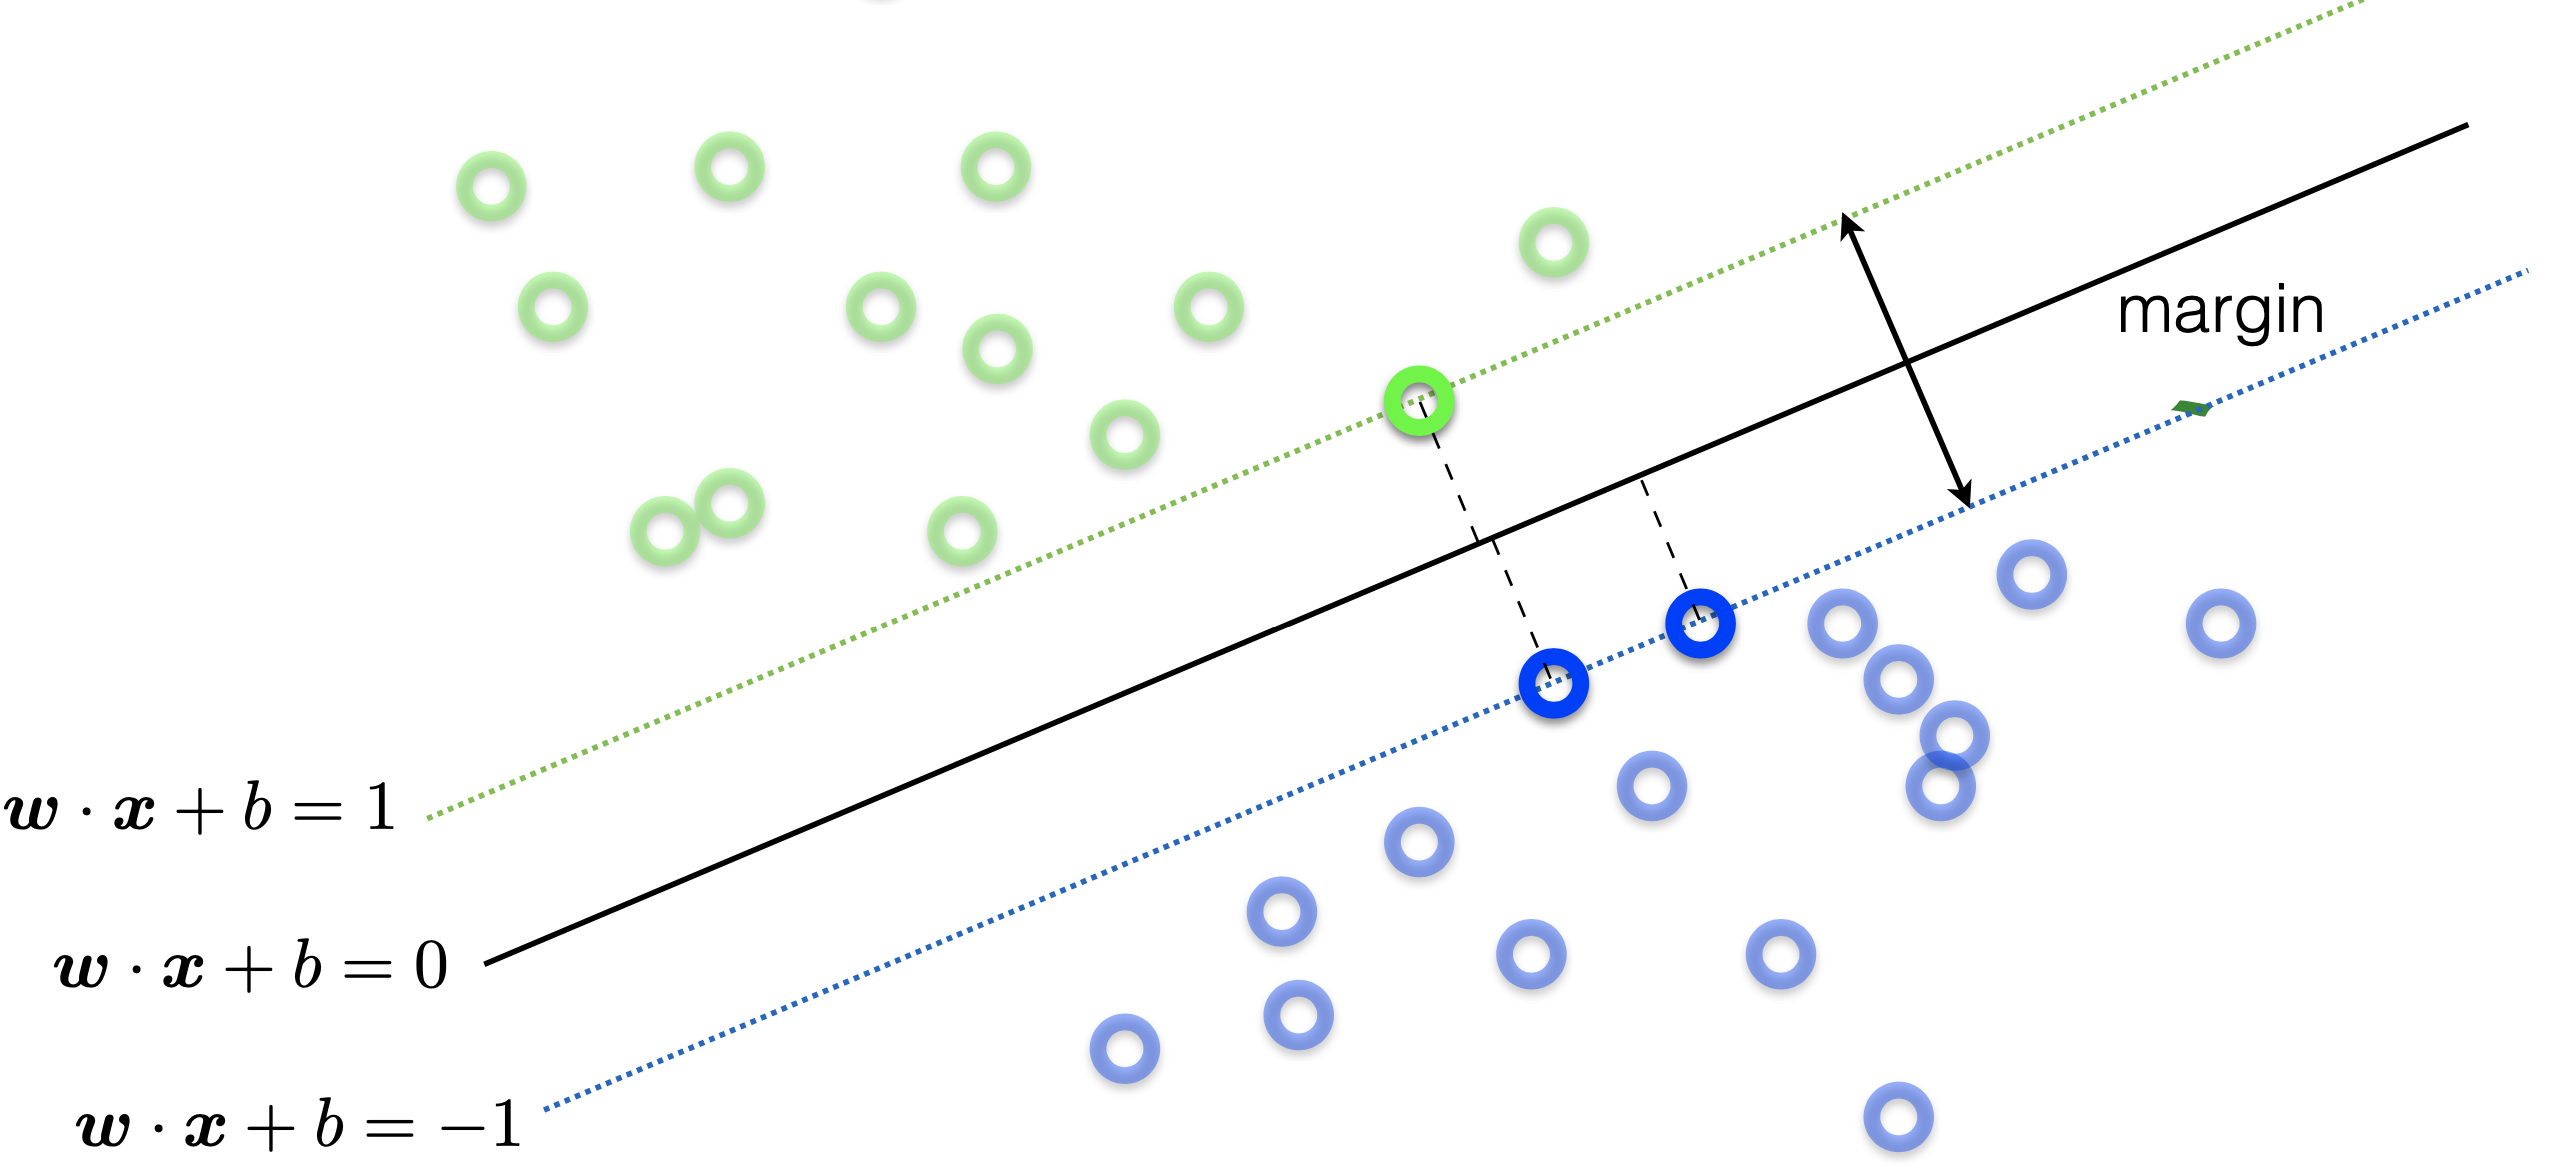
\includegraphics[width=0.6\textwidth]{images/Best Margin.png}
    \caption{Highlights the max margin classifier along with the margin hyperplanes}
    \label{fig:3}
\end{figure}

\subsection{Soft Margin SVM}

\subsection*{{\textbf{Intuition}}}\\
We saw in the previous section that SVM has to satisfy the hard constraints to converge and find a decision boundary for a separable data. But it is quite possible in real world data to have a few samples which lie very close to the samples of the opposite label as shown in Fig 4. even while maintaining data separability. In such scenarios, a hard SVM will try to find the maximum margin from the nearest sample and the decision boundary will look like as given in Fig 4. This brings us to the intuition that if we relax our constraints a bit and allow some misclassification, we can find a better margin. This is the notion of soft margin. 
\begin{center}
    \textit{We should allow for some misclassification if we can get more robust classification}
\end{center}

\begin{figure}[!htp]
  \centering
  \begin{minipage}[b]{0.4\textwidth}
    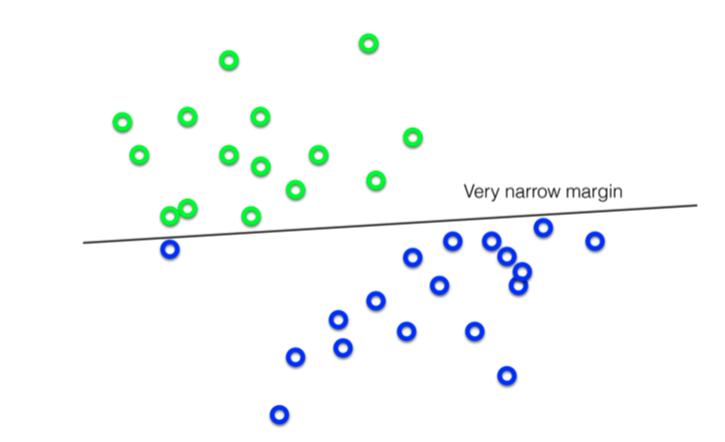
\includegraphics[width=\textwidth]{images/HardMargin.png}
    \caption{Hard Margin}
  \end{minipage}
  \hfill
  \begin{minipage}[b]{0.4\textwidth}
    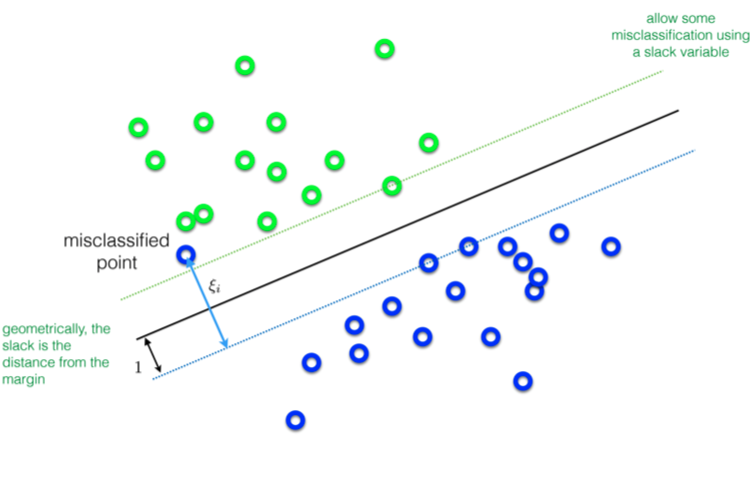
\includegraphics[width=\textwidth]{images/xiDefinition.png}
    \caption{Soft Margin with \(\xi\)}
  \end{minipage}
   
    \end{figure}


\subsection*{{\textbf{Slack Variable}}}\\
To allow this tradeoff between the margin and the mistakes, a slack variable is introduced in the constraint. The slack variable \(\xi_{i}\) is defined as the distance of the point from the margin as shown in Fig 5. We can control the extent of mistakes allowed by our algorithm by this parameter \(\xi_{i}\). After including this variable, our hard constraint tranforms into a soft constraint that allows some mis-classification as, 
\begin{gather*}
   y_{i}(w^Tx_{i}+b) \geq 1 - \xi_{i} \\
\text{where \(\xi_{i} \geq 0\)}  
\end{gather*}

\subsection*{{\textbf{Objective Function}}}

Following from our previous objective function in hard constraint case, now we need to minimize the sum of \(\xi_{i}\) along with the weight vector. Hence our objective function becomes, 
\begin{gather*}
    min_{w, \xi}(\norm{w}^2 + C\sum_{i} \xi_{i}) \\
    \text{subject to} \\
    y_{i}(w^Tx_{i}+b) \geq 1 - \xi_{i} \\
    \text{for i = 1 to N}  
\end{gather*}

We can see from the objective function that 
\begin{enumerate}
    \item If C tends to infinity, we end up giving a lot of weight to minimize the mistakes and thus the problem converts to hard margin case.
    \item If we reduce C to a very small value , the optimization function ends up reducing the weight vector towards 0
\end{enumerate}
Hence, C can be chosen as a value in between for instance 10. In this case it will be termed as a soft margin.

Now to incorporate linear constraints into the objective function, we replace the value of \(\xi_{i}\) from the inequality and put it in the objective function.
\begin{align}
    min_{w}(\frac{\lambda}{2}\norm{w}^2 + \frac{1}{M}\sum_{i=0}^{M} 1- y_{i}w^Tx_{i}) \label{eq11}
\end{align}
where, \(\lambda\) is an inverse multiplier at the place of C \\
M = number of training samples

In the equation \ref{eq11} we have included \(\xi\) of all the points to minimize without any added constraint. This creates problem by making the second term negative when more number of points are correctly classified (easy examples). This overpowers the loss from wrongly identified points and thus fail to generalize. 

\begin{figure}[!htp]
        \centering
        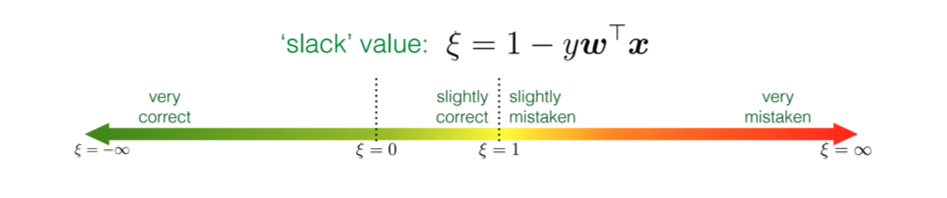
\includegraphics[width=\textwidth]{images/xiRange.png}
        \caption{Spectrum of \(\xi\) and its interpretation}
\end{figure}

Since we do not gain by minimizing the loss on easy examples, we can avoid them all together and concentrate on the region where our point is slightly correct, slightly mistaken or very mistaken. As can be seen in Fig 6, such region corresponds to \(\boldsymbol{\xi > 0}\). 
This observation motivates us to clip the values of \(\xi < 0\) in the objective function. And thus we can replace the second part of the objective function with a \textbf{Hinge Loss} which is defined as,
\begin{align}
     Hinge Loss = max(0, 1- y_{i}w^Tx_{i}) \label{eq12}
\end{align}
Substituting equation \ref{eq12} in \ref{eq11} we get our final objective function as, 
\begin{align}
     min_{w}(\underset{\mathclap{\substack{\\ \\ \textstyle \text{\textbf{regularization}}}}}{\frac{\lambda}{2}\norm{w}^2}+\underset{\mathclap{\substack{\\ \textstyle \text{\textbf{loss function}}}}}{\frac{1}{M}\sum_{i=0}^{M} max(0, 1-y_{i}w^Tx_{i})}) \label{eq13}
\end{align}

As we can see in equation \ref{eq13}, we have finally converted our objective function to a familiar function we saw in Online Gradient Descent. \textit{\textbf{It is a linear function with a quadratic regularization.}}
\newpage
\textbf{Properties of this function}
\begin{enumerate}
    \item It is a convex function
    \item It is not differentiable because of Hinge Loss
\end{enumerate}

To solve such convex optimization problems where the function is not differentiable we can use a variant of Gradient Descent called \textbf{Online Sub-Gradient Descent}

\subsection{Sub Gradients}
\begin{figure}[!htp]
        \centering
        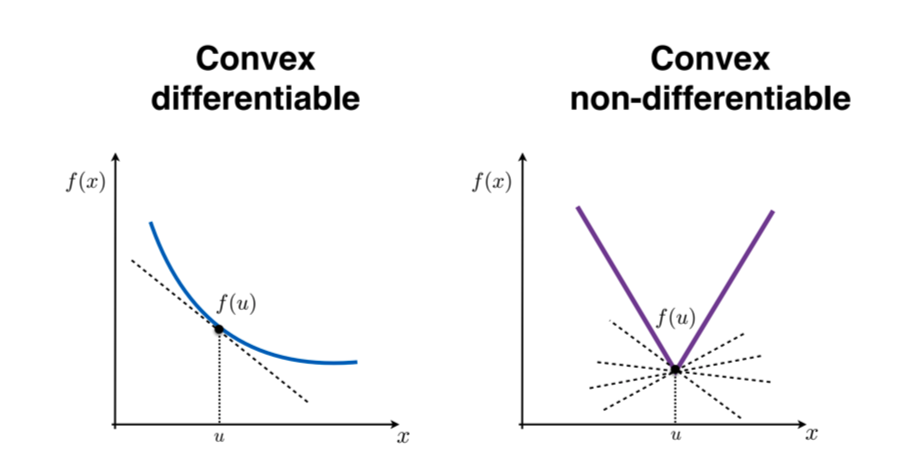
\includegraphics[width=0.7\textwidth]{images/SubGradient.png}
        \caption{Gradient and Sub-Gradient}
\end{figure}

{
\definition[Sub-Gradients\cite{subgradient}]{
The subgradient of a convex function f at \(w_{0}\) is formally defined as all vectors v such that for any other point w, \\
$$f(w) - f(w_{0}) \geq v(w - w_{0})$$
If f is differentiable at \(w_{0}\), then the subgradient contains only one vector which is the gradient \(\delta f(w_{0}\)). However, when f is not differentiable, there may be many different values for v that satisfy this inequality as shown in Fig 7.}
}\\ \\
For our problem statement, Hinge Loss is not differentiable at 0 and thus we need to use sub-gradients at that location. Since, there can be many sub-gradients, we can choose 2 sub-gradients based on the direction of the function. One for the part of the function greater than 0 and one for the part less than 0. 
\begin{align}
    z_{m} = 
    \left\{
        \begin{array}{ll}
            0 & \mbox{if $y_{i}w^Tx_{i} \geq 1$},\\
            -y_{i}x_{i} & \mbox{otherwise}\\   
        \end{array}
    \right.
\end{align}

Since we have all the tools required for optimization, we can solve this by using Online Sub-Gradient Descent. This algorithm works same as Online Gradient Descent as explained before but uses sub-gradients at the place of gradients.
Now we can write the complete algorithm of Soft SVM in the format of Online Mirror Descent(OMD) as this is also a special case of OMD.


\begin{algorithm}[H]
\caption{SoftSVM(\(\lambda\))}
\label{algo:softsvm}
\begin{algorithmic}[1]
\STATE $\textbf{\(\theta\)}^{(1)} \leftarrow \{0 \in R^N\}$ \hfill $\triangleright$ Weight initialization
\FOR{$t=1,\;\cdots,\;T$}
\STATE $y_{d}, \boldsymbol{x}_{d} \sim D$ \hfill $\triangleright$ Receive sample from environment
\STATE $\theta^{(t)} = \theta^{(t-1)} + y_{d}{x}_{d} . \mathbbm{1} [y_{d}(w^{(t)} . x_{d}) < 1] $ 
\hfill $\triangleright$ Dual parameter update
\STATE $w^{(t+1)} \leftarrow \frac{1}{\lambda+1} \theta^{(t)}$ \hfill $\triangleright$ Mirror projection
\ENDFOR
\STATE $w = \frac{1}{T}\sum_{t} w^{t} $
\end{algorithmic}
\end{algorithm}

\subsection{Comparison of Soft SVM with Perceptron Algorithm}

\begin{algorithm}[H]
\caption{Perceptron Algorithm}
\label{algo:softsvm}
\begin{algorithmic}[1]
\STATE $\textbf{\(\theta\)}^{(1)} \leftarrow \{0 \in R^N\}$ \hfill $\triangleright$ Weight initialization
\FOR{$t=1,\;\cdots,\;T$}
\STATE RECEIVE($y^{(t)}, \boldsymbol{x}^{(t)}$) \hfill $\triangleright$ Receive sample from environment
\STATE $\theta^{(t)} = \theta^{(t-1)} + y^{(t)}{x}^{(t)} . \mathbbm{1} [y^{(t)}\langle w^{(t)} . x^{(t)}\rangle < 0] $ \hfill $\triangleright$ Dual parameter update
\STATE $w^{(t+1)} \leftarrow \theta^{(t)}$
\ENDFOR
\end{algorithmic}
\end{algorithm}

As we can see in the above algorithms
\begin{enumerate}
    \item Both the algorithms have similar dual parameter update. The only difference is that SVM uses soft margin while perceptron uses no margin.
    \item Both use similar mirror function.
\end{enumerate}


\newpage
\section{Appendix}
\subsection{Implementing SVM on linearly inseparable data}
Real life data is often linearly inseparable. However, \textbf{Cover's Theorem} states that ``pattern-classification problem cast in a high dimensional space non-linearly is more likely to be linearly separable than in a low-dimensional space" \cite{UWO_SVM_lecture}. This signifies that we can apply non-linear transformations on low-dimensional data in order to transform them to high dimensional vector space where they are more likely to be linearly separable. Consider the case of 1D data in figure \ref{fig:4} which is not separable by a linear function.
\begin{figure}[!h]
    \centering
    \vspace{-0.42cm}
    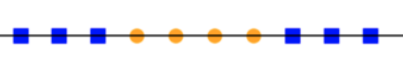
\includegraphics{images/Linear inseparable.png}
    \vspace{-1cm}
    \caption{Linearly inseparable data \cite{UWO_SVM_lecture}}
    \label{fig:4}
\end{figure}\\
We can apply a non-linear function $\phi(\mathbf{x}) = (\mathbf{x,x^2})$ to lift it in 2D space as illustrated in figure \ref{fig:5}
\begin{figure}[!h]
    \centering
    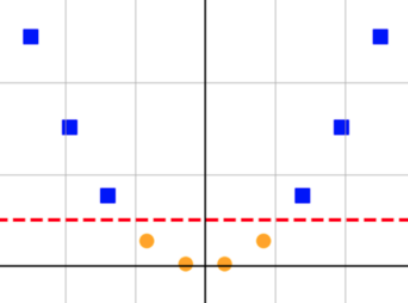
\includegraphics[width=7cm]{images/separable.png}
    \caption{Same Data made linearly separable\cite{UWO_SVM_lecture}}
    \label{fig:5}
\end{figure}\\
We can see that in this new high dimensional space, the projected data becomes linearly separable. We can then use max-margin classifier to learn a hyperplane that can separate the data points. \textbf{Kernel Tricks} is a very popular and efficient way of making a linearly inseparable data, separable. The SVM optimization function depends only on the dot product ($\mathbf{x_i^Tx_j}$) of data points and hence if we know a function $\mathbf{K}$ such that 
\[
\mathbf{K(x_i,x_j)} = \phi(\mathbf{x_i})\cdot \phi(\mathbf{x_j})
\]
then we do not explicitly need to calculate the mapping function ($\phi$) for increasing the dimension of input space. $\mathbf{K}$ is called the kernel function and calculating $\mathbf{K}$ is computationally efficient.
\newpage
%\section*{References}
%Include your references here. Please cite any resources you found useful.	
%Populate the refs.bib file or list your references manually. Be consistent in formatting!
{
\bibliography{refs}
\bibliographystyle{abbrv}
}

%\section{Appendix}
%This section provides any relevant background material that was not covered in the lectures, but was found to be useful for understanding the material. 
%For example, derivations, theory underlying techniques employed, etc. 

%Additionally, this section can summarizes applications or extensions of these techniques found in the literature. 

\end{document} % Done!


